% Step 2: RAG over the policy documents.
% Build from this folder:  tectonic learn.tex
\documentclass[11pt]{article}
% Look and feel for the Step 2 learn PDF.
% Only the typeface block changes between design variants.

\usepackage{fontspec}
\usepackage[a4paper, left=2.7cm, textwidth=13.2cm, marginparsep=0.7cm,
  marginparwidth=4.0cm, top=3.0cm, bottom=3.2cm]{geometry}
\usepackage{xcolor}
\usepackage{booktabs}
\usepackage{tabularx}
\usepackage{amsmath}
\usepackage{amssymb}
\usepackage{enumitem}
\usepackage{listings}
\usepackage{tcolorbox}
\tcbuselibrary{skins}
\usepackage{marginnote}
\usepackage{tikz}
\usetikzlibrary{arrows.meta, positioning, calc, fit, shapes.geometric}
\usepackage{caption}
\usepackage{float}
\usepackage[hidelinks]{hyperref}

% ---- typeface (the design axis) -----------------------------------
\setmainfont{lmroman10}[Extension=.otf, UprightFont=*-regular, BoldFont=*-bold, ItalicFont=*-italic, BoldItalicFont=*-bolditalic]
\newcommand{\fontlabel}{Latin Modern Roman}

\setsansfont{texgyreheros}[Extension=.otf, UprightFont=*-regular,
  BoldFont=*-bold, ItalicFont=*-italic, BoldItalicFont=*-bolditalic,
  Scale=0.88]
\setmonofont{lmmono10}[Extension=.otf, UprightFont=*-regular,
  Scale=0.92]

% ---- colours: calm neutrals, one accent ----------------------------
\definecolor{ink}{HTML}{2E2622}
\definecolor{muted}{HTML}{7A6D64}
\definecolor{line}{HTML}{DDD3C7}
\definecolor{paper}{HTML}{F6F1EA}
\definecolor{accent}{HTML}{B5583A}
\definecolor{accentbg}{HTML}{F5E6DF}

\color{ink}
\linespread{1.12}
\setlength{\parindent}{1.2em}
\setlength{\parskip}{0pt}
\emergencystretch=3em
\frenchspacing

% ---- headings ------------------------------------------------------
\makeatletter
\renewcommand\section{\@startsection{section}{1}{0pt}%
  {3.2ex plus 1ex minus .2ex}{1.6ex}%
  {\normalfont\Large\color{ink}}}
\renewcommand\subsection{\@startsection{subsection}{2}{0pt}%
  {2.6ex plus .8ex minus .2ex}{1.0ex}%
  {\normalfont\large\itshape\color{ink}}}
\renewcommand\@seccntformat[1]{%
  \llap{\color{accent}\csname the#1\endcsname\hspace{0.9em}}}
\makeatother

% ---- running head and foot ----------------------------------------
\usepackage{fancyhdr}
\pagestyle{fancy}
\fancyhf{}
\renewcommand{\headrulewidth}{0pt}
\fancyhead[L]{\footnotesize\scshape\color{muted}%
  \MakeLowercase{Step 2 \textperiodcentered{} RAG}}
\fancyhead[R]{\footnotesize\color{muted}\thepage}
\fancyheadoffset[R]{0pt}

% ---- margin notes: a short explanation of a term ------------------
\newcommand{\term}[2]{\emph{#1}\marginnote{\footnotesize\raggedright
  \color{muted}\textbf{\color{ink}#1:} #2}}
\renewcommand{\marginfont}{\footnotesize}

% ---- boxes ---------------------------------------------------------
\newtcolorbox{keypoint}{colback=accentbg, colframe=accentbg,
  boxrule=0pt, arc=0pt, left=10pt, right=10pt, top=7pt, bottom=7pt,
  borderline west={2pt}{0pt}{accent}}
\newtcolorbox{example}[1]{colback=white, colframe=line, boxrule=0.5pt,
  arc=0pt, left=10pt, right=10pt, top=6pt, bottom=6pt,
  fonttitle=\small\scshape, coltitle=muted, colbacktitle=white,
  title={\MakeLowercase{#1}}, titlerule=0.4pt, titlerule style=line}

% ---- code ----------------------------------------------------------
\lstset{
  basicstyle=\ttfamily\small,
  backgroundcolor=\color{paper},
  frame=none,
  xleftmargin=0.7em, xrightmargin=0.7em,
  aboveskip=0.9em, belowskip=0.9em,
  columns=fullflexible, keepspaces=true,
  showstringspaces=false,
  keywordstyle=\color{accent},
  commentstyle=\color{muted}\itshape,
  literate={×}{{$\times$}}1 {→}{{$\rightarrow$}}1
           {æ}{{\ae}}1 {ø}{{\o}}1 {å}{{\aa}}1 {ü}{{\"u}}1
}
\newcommand{\code}[1]{\texttt{#1}}

% ---- captions and tables -------------------------------------------
\captionsetup{font={small}, labelfont={sc,color=muted},
  textfont={color=muted}, labelsep=quad, justification=raggedright,
  singlelinecheck=false}
\renewcommand{\arraystretch}{1.18}

% ---- figure styles -------------------------------------------------
\tikzset{
  box/.style={draw=line, fill=white, rounded corners=3pt,
    font=\small, align=center, inner sep=6pt, minimum height=8mm},
  hot/.style={box, draw=accent, fill=accentbg},
  flow/.style={-{Stealth[length=2.2mm]}, draw=muted, line width=0.6pt},
  hotflow/.style={-{Stealth[length=2.2mm]}, draw=accent,
    line width=0.8pt},
  lbl/.style={font=\footnotesize, text=muted, align=center},
}

\raggedbottom


\begin{document}

\thispagestyle{empty}
\setlength{\parindent}{0pt}
\vspace*{1.2cm}
{\color{muted}\scshape\MakeLowercase{Nordhjem store}
  \textperiodcentered{} \MakeLowercase{Step 2}}\par
\vspace{0.9cm}
{\fontsize{28}{32}\selectfont RAG: answers\\[2pt] from documents\par}
\vspace{0.5cm}
{\large\itshape\color{muted} Find the right paragraphs first,\\
  then let a model write the answer\par}
\vspace{0.6cm}
{\color{accent}\rule{2.2cm}{1.2pt}}\par
\vspace{0.6cm}
\begin{minipage}{11.5cm}
\small\color{muted}
The chat on the shop answers policy questions with a keyword
placeholder: it shows the paragraph that shares the most words with the
question. In this step you replace it with RAG in \code{api/rag.py}.
The first half is your Step 1 search, reused. The second half is new:
a text model that writes an answer from what was found, and says ``I
don't know'' when nothing was.
\end{minipage}
\vspace{1.0cm}

{\small
\renewcommand{\contentsname}{\normalsize\scshape\color{muted}
  \MakeLowercase{Contents}}
\tableofcontents}

\newpage
\setlength{\parindent}{1.2em}

% ====================================================================
\section{What RAG is}

\subsection{Two ways a model can answer}

Ask a text model ``How many days do I have to return a sofa?'' and it
will answer. But from what? It has read a lot of the internet, so it
will give a typical number, maybe 30, maybe 14. It does not know
Nordhjem's rules, and it does not say that it does not know. It
\emph{sounds} sure either way. Inventing a fact in a confident voice is
called a \term{hallucination}{a fluent, confident answer that is not
true, because the model made it up.}.

The fix is to hand the model the rules with the question, and tell it
to answer only from them. Like an open-book exam: the student still
writes the answer, but from the book on the table, not from memory.

\subsection{Retrieval, then generation}

The shop has 23 policy documents, about 2\,500 words. Sending all of
them with every question would work today, but not with 2\,000
documents, and the more text a model gets, the easier it misses the one
line that matters. So the right paragraphs are \emph{found} first.

That is \term{RAG}{retrieval-augmented generation: find relevant text,
add it to the prompt, then generate the answer.}, in three words:
\begin{itemize}[leftmargin=1.4em, itemsep=2pt]
\item \textbf{Retrieval}: find the few paragraphs closest to the
  question. This is your Step 1 semantic search, on paragraphs instead
  of products.
\item \textbf{Augmented}: put those paragraphs into the prompt, with
  the question.
\item \textbf{Generation}: the text model writes the answer from them,
  and names its sources.
\end{itemize}

\begin{figure}[H]
\centering
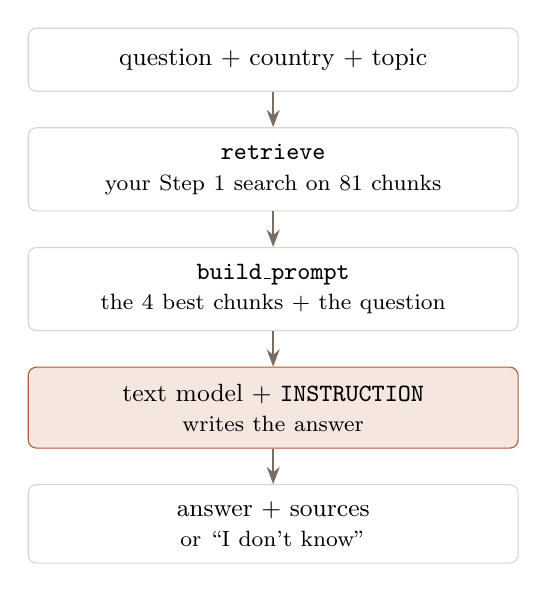
\begin{tikzpicture}[node distance=4.5mm and 6mm]
  \node[box, text width=58mm] (q) {question + country + topic};
  \node[box, below=of q, text width=58mm] (r)
    {\code{retrieve}\\ \footnotesize your Step 1 search on 81 chunks};
  \node[box, below=of r, text width=58mm] (p)
    {\code{build\_prompt}\\ \footnotesize the 4 best chunks + the question};
  \node[hot, below=of p, text width=58mm] (g)
    {text model + \code{INSTRUCTION}\\ \footnotesize writes the answer};
  \node[box, below=of g, text width=58mm] (a)
    {answer + sources\\ \footnotesize or ``I don't know''};
  \draw[flow] (q) -- (r);
  \draw[flow] (r) -- (p);
  \draw[flow] (p) -- (g);
  \draw[flow] (g) -- (a);
\end{tikzpicture}
\caption{RAG in the shop. Only the highlighted step is new in kind.}
\end{figure}

\subsection{Semantic search and RAG side by side}

\begin{table}[H]
\small
\begin{tabularx}{\textwidth}{@{}l X X@{}}
\toprule
 & Semantic search (Step 1) & RAG (Step 2) \\
\midrule
Searches over & 500 products & 81 paragraphs of policy \\
Returns & a list of products & a written answer and its sources \\
Who reads the results & the customer & the text model, then the
  customer \\
Worst failure & a wrong product in the list & a wrong answer that sounds
  right \\
\bottomrule
\end{tabularx}
\end{table}

The last row is why this step has more rules. A wrong product in a list
is easy to skip. A wrong answer in a confident sentence is believed.

% ====================================================================
\section{The documents and their chunks}

\subsection{A policy document}

The documents are in \code{data/policies/}. Each starts with a header,
then Markdown text with \code{\#\#} headings:
\begin{lstlisting}
---
doc_id: delivery-no
title: Delivery in Norway
topic: delivery
country: NO
valid_from: 2026-01-01
---
# Delivery in Norway
## Price and time
- Standard delivery: **799 NOK**. There is no free delivery ...
## Returns from Norway
...
\end{lstlisting}

\subsection{Chunks}

A whole document is too coarse to retrieve: ``Delivery in Norway''
covers price, customs and returns. A single sentence is too fine: it
loses its context. Here a \term{chunk}{the unit that is embedded and
retrieved: one piece of a document.} is one heading with its
paragraphs. The 23 documents give 81 chunks.

\code{loaders/load\_policies.py} has already embedded every chunk (as
\code{RETRIEVAL\_DOCUMENT}, normalised, like the products) and stored
it in Firestore, in the collection \code{policy\_chunks}. The embedded
text includes the title and the heading, because a heading like ``Price
and time'' means little without ``Delivery in Norway'':
\begin{lstlisting}
Delivery in Norway. Price and time.
- Standard delivery: **799 NOK**. There is no free delivery ...
\end{lstlisting}

\code{load\_chunks} in \code{api/rag.py} reads them into a
\code{ChunkIndex}, the same idea as your \code{Index}: row~i of every
list is chunk~i. It is given, since you wrote one already.

% ====================================================================
\section{Retrieval with rules}

\subsection{Meaning is not enough}

Some chunks must never reach the model, however close they are in
meaning:
\begin{itemize}[leftmargin=1.4em, itemsep=2pt]
\item \textbf{Another country.} A customer in Sweden asks ``How much is
  delivery?''. The Danish chunk (499~kr) is as close in meaning as the
  Swedish one (599~SEK). Only the Swedish one may be used.
\item \textbf{An old version.} \code{returns-2025} (30 days) was
  replaced by \code{returns-2026} (60 days). Both answer ``how long can
  I return?'' equally well. Only the current one is true.
\end{itemize}
These are filters, exactly like \code{filter\_products}: a yes or no
per chunk, applied before ranking. That is TODO~1,
\code{allowed\_chunks}.

\begin{lstlisting}
                  countries  valid_to     DK on 2026-11-13
returns-2026      [all]      None         True
delivery-dk       [DK]       None         True
delivery-se       [SE]       None         False   other country
returns-2025      [all]      2025-12-31   False   expired
\end{lstlisting}

\begin{keypoint}
Dates written year-month-day compare correctly as plain text:
\code{"2025-12-31" < "2026-11-13"} is \code{True}. No date objects
needed.
\end{keypoint}

\subsection{The topic: a preference, not a filter}

The chat lets the customer pick a topic, such as \emph{Returns}. It
would be natural to filter on it. But the test question ``How much is a
return pickup in Norway?'' is a returns question whose answer is in
\emph{Delivery in Norway}. A topic filter would hide it.

So the topic only adds a small bonus to the score of chunks in that
topic: \code{TOPIC\_BONUS = 0.03}. A chunk in the right topic moves up;
a much better chunk elsewhere still wins.
\begin{lstlisting}[language=Python]
scores = scores + TOPIC_BONUS * (index.topics == topic)
\end{lstlisting}
\code{index.topics == topic} gives True or False per chunk; times a
number, True counts as 1 and False as 0.

\subsection{\code{retrieve}}

TODO~2 is your Step 1 \code{search} again: embed, normalise, score with
\code{@}, add the topic bonus, \code{np.where} with $-\infty$ for the
chunks that are not allowed, cap $k$, \code{get\_top\_k}. The functions
from \code{api/search.py} are imported, so you reuse your own code.
\code{K = 4}: the four best chunks go to the model.

% ====================================================================
\section{The prompt}

The model gets two texts. The \emph{instruction} (TODO~4) is the same
for every question. The \emph{prompt} (TODO~3) changes each time:
\begin{lstlisting}
Customer's country: Norway (NO)

Sources:
[delivery-no] Delivery in Norway, Returns from Norway
You have the same 60 days to return an item. A return pickup in
Norway costs **599 NOK**. ...

[returns-2026] Returns policy, Cost of returning
Returning an item in a store is free. ...

Question: How much is a return pickup in Norway?
\end{lstlisting}

Three things in it do real work:
\begin{itemize}[leftmargin=1.4em, itemsep=2pt]
\item \textbf{The country.} The chunks were already filtered by
  country, but a chunk for ``all'' can still mention several countries
  (the warranty chunk has both 2 and 5 years). The model needs to know
  which applies.
\item \textbf{The \code{[doc\_id]} labels.} The model answers with the
  ids it used. That is how the chat shows ``Source: Delivery in
  Norway''.
\item \textbf{Several chunks.} Some answers need two: ``Can I return a
  mattress after 80 nights?'' needs the trial, which overrides the
  normal returns rule.
\end{itemize}

% ====================================================================
\section{The instruction: being honest}

The instruction decides whether the model stays inside the sources.
The rules that matter most:

\begin{table}[H]
\small
\begin{tabularx}{\textwidth}{@{}X X@{}}
\toprule
Rule & Without it \\
\midrule
answer only from the sources & ``Do you offer interior design?'' gets
  a friendly, invented yes \\
if they do not answer, say ``I don't know'' & the model fills the gap
  from what shops usually do \\
list the doc\_ids used & no way to show or check the source \\
use the customer's country & the Danish 2-year rule for a Norwegian
  customer \\
answer in the question's language & a Danish question gets English \\
\bottomrule
\end{tabularx}
\end{table}

\begin{keypoint}
``I don't know'' is a right answer. Three test questions have no answer
in the documents, and they pass only if the chat says so. Retrieval
always returns four chunks, even for a question about renting
furniture: only the instruction stops the model from building an answer
out of whatever came back.
\end{keypoint}

\subsection{The answer as a form}

As in Step 1b, the model fills in a form instead of writing free text:
\begin{lstlisting}[language=Python]
class RagAnswer(BaseModel):
    answer: str
    sources: list[str]     # doc_ids, for example ["delivery-no"]
\end{lstlisting}
The model can still write an id that was not in the prompt. So
\code{answer} keeps only ids that were among the retrieved chunks, and
turns each into a \code{Source} with its title.

% ====================================================================
\section{The exercise}

Everything is in \code{api/rag.py}. Work from top to bottom:

\begin{enumerate}[leftmargin=1.4em, itemsep=3pt]
\item \textbf{TODO 1}, \code{allowed\_chunks}: country and dates, one
  True or False per chunk (section~3.1).
\item \textbf{TODO 2}, \code{retrieve}: your Step 1 search with the
  topic bonus (sections~3.2 and~3.3).
\item \textbf{TODO 3}, \code{build\_prompt}: the text in section~4.
\item \textbf{TODO 4}, \code{INSTRUCTION}: the rules in section~5.
\item \textbf{TODO 5}, \code{answer}: retrieve, build the prompt, ask
  the model, turn the ids into sources.
\end{enumerate}

Check your work from the repo root:
\begin{lstlisting}
python3 steps/02_rag/check.py
\end{lstlisting}
\begin{itemize}[leftmargin=1.4em, itemsep=2pt]
\item \textbf{Part 1} tests \code{allowed\_chunks} and
  \code{build\_prompt} on four made-up chunks, without Google.
\item \textbf{Part 2} tests retrieval: for each of the 27 answerable
  questions, is a right document among the four chunks? Pass mark 90\,\%,
  and the expired 2025 policy must never come back.
\item \textbf{Part 3} asks the full RAG all 30 questions. An answer
  passes when it has the key fact (``60'', ``599'') and a right source.
  Pass mark 85\,\%, and all three no-answer questions must get ``I don't
  know''.
\end{itemize}
The reference solution in this folder passes with 27 of 27 found and 27
of 27 answers right.

% ====================================================================
\section{Experiments, after it passes}

\begin{itemize}[leftmargin=1.4em, itemsep=3pt]
\item Remove the ``I don't know'' rule from your instruction. What does
  the chat say about renting furniture?
\item Set \code{K = 1}. Which questions break? (Look at the ones of kind
  \code{two\_docs}.)
\item Turn the topic bonus into a hard filter, pick \emph{Returns} and
  ask about the return pickup in Norway.
\item Remove the date check from \code{allowed\_chunks} and ask ``Is the
  return period still 30 days?''.
\item Ask in Danish or German. Does the answer follow your language?
\end{itemize}

\end{document}
